\documentclass{article}
\usepackage[utf8]{inputenc}
\usepackage{siunitx}
\usepackage{graphics}
\usepackage[american,siunitx]{circuitikz}
\usepackage{amsmath}
\usepackage{svg}
\usepackage{booktabs}
\usepackage{float}
\usepackage{xparse, xfp}
\usepackage{graphicx} 
\usepackage{steinmetz}
\usepackage{hyperref}
\renewcommand{\thesubsubsection}{\thesubsection.\alph{subsubsection}}
\newcommand{\equal}{=}

\title{ECE2101L\\Electrical Circuit Analysis II Laboratory\\\,\\Lab 8\\ Op Amp in AC Circuits\\\,\\Report\\}
\author{Choi Tim Antony Yung}
%\author{Choi Tim Antony Yung\\\,\\Willis Nguyen\\Phineas Cozmiuc}

\begin{document}

\clearpage\maketitle
\thispagestyle{empty}
\newpage
\setcounter{page}{1}

\section{Basic characteristics of non-inverting positive-gain op amp circuit}
\begin{center}
    \begin{circuitikz}
        \draw 
            (0, 0) node[op amp, yscale=-1] (opamp) {}
            (opamp.+) to[short] ++(-0.01,0) -- ++(-2.99,0) to[sinusoidal voltage source,l_=$v_s(t)$] ++(0,-5) coordinate (groundnode) node[ground]{}
            (opamp.-) to[short] ++(-0.01,0) -- ++(-0.34,0) -- ++(0,-2) coordinate (vnnode)
            -- (vnnode -| opamp.-) to[R,l_=$R_f$] (vnnode -| opamp.out)
            (groundnode) -- (groundnode -| vnnode) to[R=$R_g\equal\SI{1300}{\ohm}$] (vnnode)
            (opamp.out) -- ++(0.5,0) coordinate (outnode)
            (vnnode -| opamp.out) -- ++(0.5,0) to[short,i<=$i(t)$] (outnode) -- ++(1.5,0) coordinate (vnaughtplusnode)
            (groundnode -| vnnode) -- (groundnode -| vnaughtplusnode) to[open, v^<=$v_o(t)$] (vnaughtplusnode)
            % op amp pinout label
            (opamp.down) to[open] ++ (0,0.15) node[anchor=south east, color=red] {7}
            (opamp.up) ++ (0,-0.15) node[anchor=north east, color=red] {4}
            (opamp.+) node[anchor=north west, color=red] {3}
            (opamp.-) node[anchor=south west, color=red] {2}
            (opamp.out) ++(-0.15,0) node[anchor=south east, color=red] {6}
            ;
    \end{circuitikz}
\end{center}
\subsection*{Theory}
Assuming ideal op amp, no current is flowing into inverting input and there is no voltage difference between inverting and non-inverting input, therefore i is both the current flowing across $R_f$ and across $R_g$ and voltage at inverting input is $v_s$. Then:
$$i=\frac{v_s}{R_g}$$
$$v_o=iR=\frac{v_s}{R_g}(R_f+R_g)=(\frac{R_f}{R_g}+1)v_s$$
$$G=\frac{v_o}{v_s}=(\frac{R_f}{R_g}+1)\frac{v_s}{v_s}=\frac{R_f}{R_g}+1$$
For sinusoidals:
$$v_{rms}=\frac{v_{peak}}{\sqrt{2}}\quad i_{rms}=\frac{i_{peak}}{\sqrt{2}}$$

\subsection*{Procedure}
The above circuit was simulated with LTspice XVI as follow. The obtained measurements of voltage and current are then divided by $\sqrt{2}$ to obtain the below results.
\begin{figure}[H]
    \centering
        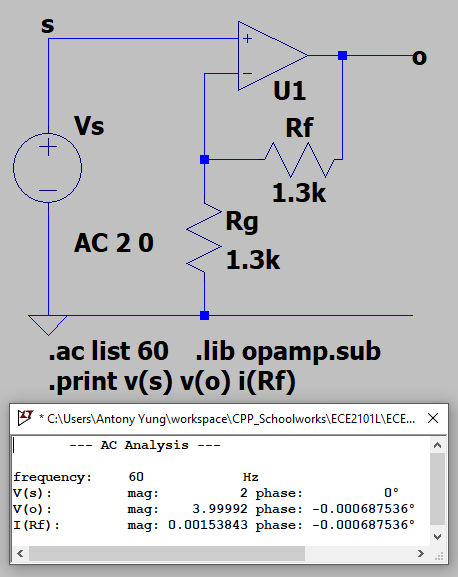
\includegraphics[scale=1]{ECE2101L_Lab08_B1_1300.png}
        \caption{Screenshot of circuit description used and the simulation result with $R_f=\SI{1.3}{\kilo\ohm}$}
\end{figure}
\begin{figure}[H]
    \centering
        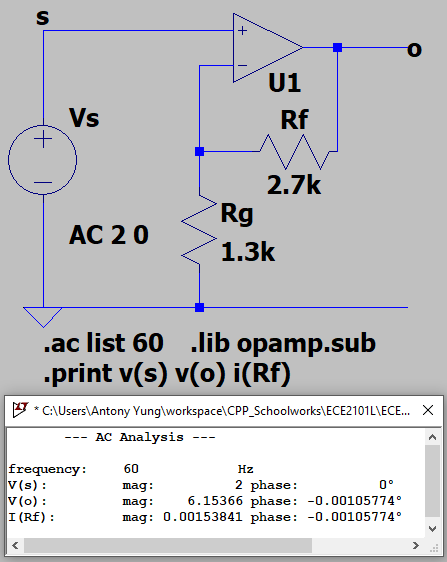
\includegraphics[scale=1]{ECE2101L_Lab08_B1_2700.png}
        \caption{Screenshot of circuit description used and the simulation result with $R_f=\SI{2.7}{\kilo\ohm}$}
\end{figure}
\begin{figure}[H]
    \centering
        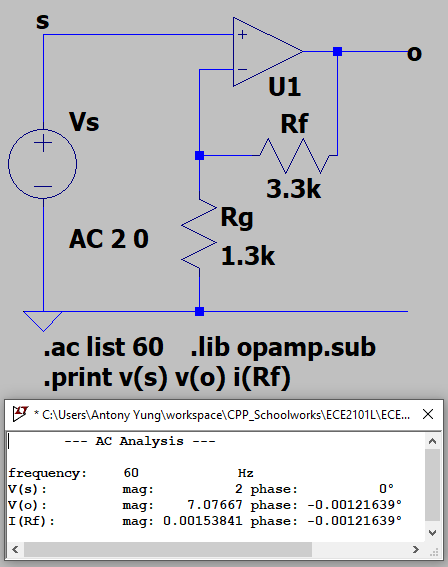
\includegraphics[scale=1]{ECE2101L_Lab08_B1_3300.png}
        \caption{Screenshot of circuit description used and the simulation result with $R_f=\SI{3.3}{\kilo\ohm}$}
\end{figure}

\newpage

\subsection*{Result}
\begin{table}[H]
    \resizebox{\columnwidth}{!}{%
    \begin{tabular}{cccccccc}
        \toprule
        $R_f$ & $V_o$ RMS & G & $V_s$ RMS & $V_o$ RMS & $I$ RMS & G & G \\
        & calculated & calculated & measured & measured & measured & measured & error \\
        \midrule
        \SI{1300}{\ohm} & \SI{2.82843}{\volt} & 2.00000 & \SI{1.41421}{\volt} & \SI{2.82837}{\volt} & \SI{0.00108783}{\ampere} & 1.99996 & 0.00\% \\
        \SI{2700}{\ohm} & \SI{4.35143}{\volt} & 3.07692 & \SI{1.41421}{\volt} & \SI{4.35130}{\volt} & \SI{0.00108782}{\ampere} & 3.07683 & 0.00\% \\
        \SI{3300}{\ohm} & \SI{5.00414}{\volt} & 3.53846 & \SI{1.41421}{\volt} & \SI{5.00396}{\volt} & \SI{0.00108782}{\ampere} & 3.53834 & 0.00\% \\
        \bottomrule    
    \end{tabular} }
\end{table}

\subsection*{Analysis}
As the circuit was simulated instead of built physically, the error demostrated by the simulation is close to zero. The non-zero error could be due to the methodology of which the simulator simulates the circuit. If this is a physical circuit, non-ideal components and imprecise measurements can contributes to error.

Assuming ideal op amp, no current flow into the inverting input of op amp, and therefore current flowing across $R_g$ must be the same as I, current flowing across $R_f$, by KCL. As the current flowing across $R_g$ is $\frac{V_-}{R_g}=\frac{V_s}{R_g}$ which does not depend on the value of $R_f$, I must remain constant as well.

\newpage

\section{Complex gain of inverting op amp circuit}
\begin{center}
    \begin{circuitikz}
        \draw 
            (0, 0) node[op amp] (opamp) {}
            (opamp.-) -- ++(-0.5,0) to[R,l_=$R_1\equal\SI{1.3}{\kilo\ohm}$] ++(-2.5,0) to[V,l_=$V_s$] ++(0,-2) -- ++(2,0) node[circ]{} node[ground](groundnode){} -- (groundnode |- opamp.+) -- (opamp.+)
            (opamp.-) ++(-0.5,0) -- ++(0,1) coordinate (tempcoor) 
            (tempcoor -| opamp.out) to[R,l_=$R_2\equal\SI{4.3}{\kilo\ohm}$] (tempcoor) -- ++(0,1.25) coordinate(temptempcoor) to[C,l=$C_2\equal\SI{0.1}{\micro\farad}$]  (temptempcoor -| opamp.out) -- (tempcoor -| opamp.out)
            (tempcoor -| opamp.out) -- (opamp.out) -- ++(1.5,0) coordinate (voplus) to[open, v=$V_o$] (voplus |- groundnode) -- (groundnode)
            
            % op amp pinout label
            (opamp.down) node[anchor=north, color=red] {7}
            (opamp.up) node[anchor=south, color=red] {4}
            (opamp.+) node[anchor=north west, color=red] {3}
            (opamp.-) node[anchor=south west, color=red] {2}
            (opamp.out) ++(-0.15,0) node[anchor=south east, color=red] {6}
            ;
    \end{circuitikz}
\end{center}
\subsection*{Theory}
The complex gain can be determined as follow:
$$G=\frac{V_o}{V_s}=-\frac{Z_2}{Z_1}=-\frac{R_2||Z_{C_2}}{R_1}=-\frac{\frac{1}{\frac{1}{R_2}+Z_{C_2}}}{R_1}=-\frac{1}{\frac{R_1}{R_2}+R_1Z_{C_2}}=\frac{-\frac{R_1}{R_2}+R_1\omega C_2j}{(\frac{R_1}{R_2})^2+(R_1\omega C_2)^2}$$
$$G=-\frac{1}{\frac{1300}{4300}+(1300)(2\pi120)(0.1)(10^{-6})j}=-2.993+0.9704j=3.1465\phase{162.0367^{\circ}}$$

\subsection*{Result}
\begin{table}[H]
    \resizebox{\columnwidth}{!}{%
    \begin{tabular}{cccccccc}
        \toprule
        Partner & G & $V_o$ RMS & $V_o$ RMS & $V_o$ \\
        & calculated & calculated & measured & error\\
        \midrule
        3 & 3.1465\phase{162.0367^{\circ}} & 4.44976\phase{162.0367^{\circ}}V & 4.44953\phase{162.034^{\circ}}V & 0.00\% \\
        \bottomrule
    \end{tabular} }
\end{table}

\section{Changing phase shift using op amp circuit}
$$G=\frac{-\frac{R_1}{R_2}+R_1\omega \frac{C_2}{10}j}{(\frac{R_1}{R_2})^2+(R_1\omega \frac{C_2}{10})^2}=3.3060\phase{178.1431^{\circ}}$$
Currently the op amp applys a $162.034^{\circ}$ phase shift to the source voltage. As the gain phasor is in the second quadrant, as we decrease the positive reactance, the phase of gain phasor will increase. As seen in the above calculation, reducing $C_2$ by a factor of 10 will increase the phase shift the op amp applys to the source voltage from $162.0367^{\circ}$ to $178.1431^{\circ}$, an increase larger than $10^{\circ}$. This is verified by the below simulation shown in figure 5.
\begin{figure}[H]
    \centering
        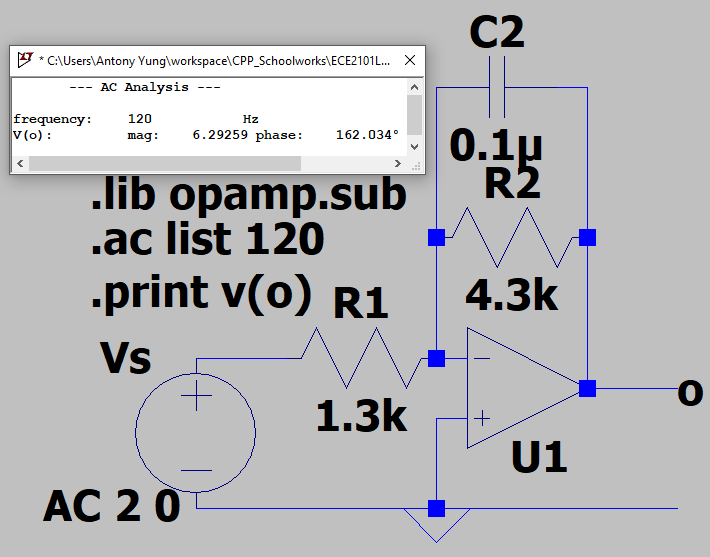
\includegraphics[scale=0.55]{ECE2101L_Lab08_B2.png}
        \caption{Screenshot of circuit description used and the simulation result}
\end{figure}
\begin{figure}[H]
    \centering
        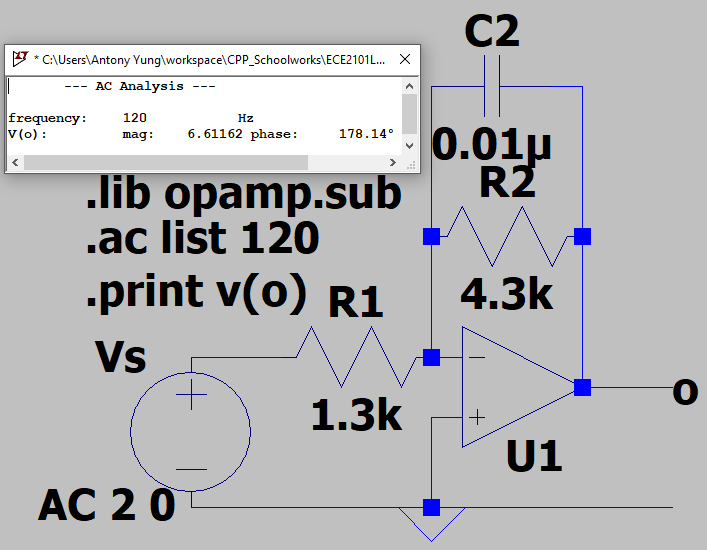
\includegraphics[scale=0.55]{ECE2101L_Lab08_B3.png}
        \caption{Screenshot of circuit description used and the simulation result}
\end{figure}

\end{document}

